\documentclass{article}
\usepackage[margin=1in]{geometry} % For setting page margins
\usepackage{amsmath}
\usepackage{amssymb} % For math symbols and equations
\usepackage{graphicx} % For including images
\usepackage{hyperref} 
\usepackage{enumitem}
\usepackage{float}
\usepackage{listings}
\usepackage{xcolor}
\usepackage{caption}

\renewcommand{\thesection}{\arabic{section}.}
\renewcommand{\thesubsection}{(\alph{subsection})}

\lstdefinestyle{matlabstyle}{
    language=Matlab,              % Specify the language
    basicstyle=\ttfamily\footnotesize\color{black}, % Code font
    keywordstyle=\color{blue}\bfseries, % Keywords in blue
    stringstyle=\color{orange},    % Strings in green
    commentstyle=\color{magenta}, % Comments in magenta
    numbers=left,                 % Line numbers on the left
    numberstyle=\tiny\color{black},% Line number style
    stepnumber=1,                 % Line number increment
    breaklines=true,              % Line breaking
    frame=single,                 % Border around code
    backgroundcolor=\color{white},
    tabsize=4,                    % Tab size
    showstringspaces=false,       % Don't show spaces in strings
}

\begin{document}

\title{
    \begin{tabular}{@{}l@{}}
        \textbf{Class:} Robust Multivariate Control \\
        \textbf{Professor:} Dr. Sean Humbert \\
        \textbf{TAs:} Santosh Chaganti \\
        \textbf{Student:} Steve Gillet \\
        \textbf{Date:} \today \\
        \textbf{Assignment:} Homework 5
    \end{tabular}
}

\author{}
\date{}

\maketitle

\section{}

\textit{For the simple SISO negative feedback system with \(P(s) = \frac{1}{s-1}\) and \(C(s) = \frac{s-1}{s+2}\), show that at least one transfer function from exogenous signals \(r\) and \(d_I\) to the internal signals \(e\), \(u\) and \(y\) is unstable due to the right-half plane pole/zero cancellation of \(s - 1\) in the loop transfer function \(L = PC\).}

\begin{figure}[H]
    \centering
    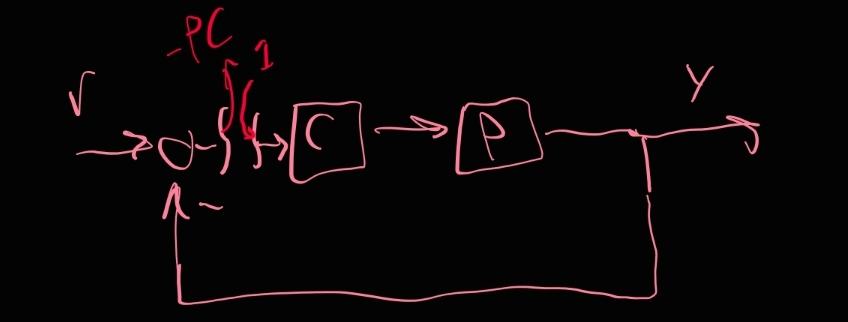
\includegraphics[width=\textwidth]{p1ryDiagram.jpg}
\end{figure}

I will start with the transfer function from \(r\) to \(y\) which for this SISO unity feedback system is:
\[
\frac{PC}{1 + PC}
\]

Or:

\[
\frac{(\frac{1}{s-1})(\frac{s-1}{s+2})}{1 + (\frac{1}{s-1})(\frac{s-1}{s+2})} = \frac{\frac{1}{s+2}}{1+\frac{1}{s+2}} = \frac{\frac{1}{s+2}}{\frac{s+2}{s+2}+\frac{1}{s+2}} = \frac{\frac{1}{s+2}}{\frac{s+3}{s+2}} = \frac{1}{s+3}
\]

This transfer function is not only stable but it was made stable by the addition of the controller and the pole/zero cancellation. Let us see some other signals, eh.

Full system diagram with $d_I$:

\begin{figure}[H]
    \centering
    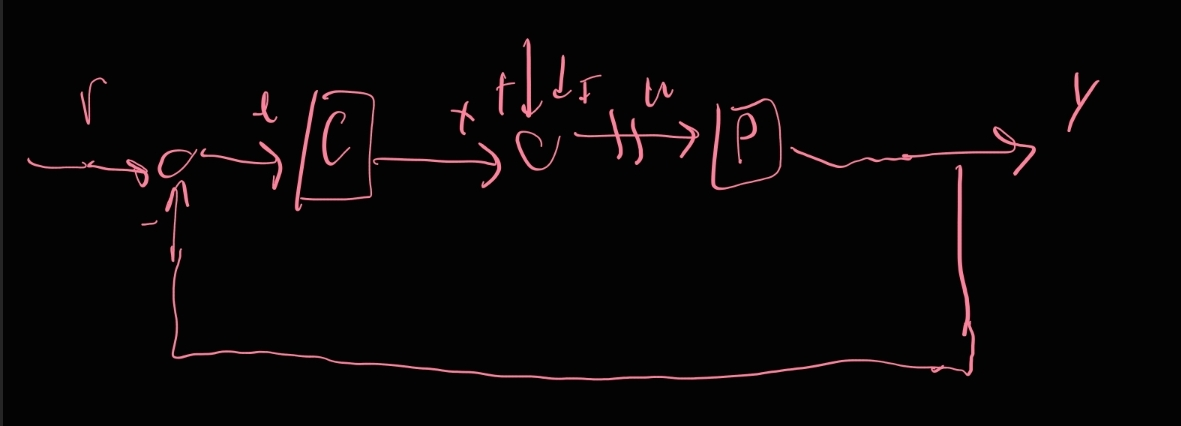
\includegraphics[width=\textwidth]{p1diyDiagram.jpg}
\end{figure}

Let's try r$\to$u:

Direct path: \(C\)
Return path: \(1 + PC\)

\[
\frac{C}{1+PC}
\]

\[
\frac{\frac{s-1}{s+2}}{1 + \frac{1}{s-1}\frac{s-1}{s+2}} =
\]

\[
\frac{\frac{s-1}{s+2}}{1 + \frac{1}{s+2}} = \frac{\frac{s-1}{s+2}}{\frac{s+3}{s+2}} = \frac{s-1}{s+3}
\]

\[
= \frac{s-1}{s+3}
\]

Again the pole is at -3 and the transfer function is stable.
Let's try $d_I \rightarrow y$:

\[
\frac{P}{1 + CP}
\]

\[
\frac{\frac{1}{s-1}}{\frac{s+3}{s+2}}
\]

\[
= \frac{s+2}{(s-1)(s+3)}
\]

There we go, a pole at $s = 1$, the transfer function from $d_I$ to y is unstable.

\section{}

\textit{For the following longitudinal model for an F-4 Phantom with 4 perturbation states (pitch rate \(\Delta q\), forward speed \(\Delta u\), angle of attack \(\Delta \alpha\), pitch angle \(\Delta \theta\)), 2 inputs (elevator deflection \(\Delta \delta_e\), flaperon deflection \(\Delta \delta_f\)) and 2 outputs (\(\Delta q\) and \(\Delta \alpha\)). Note that the \(D\) matrix entries are zeros for this output selection.}

\[
A = \begin{pmatrix}
-0.8 & -0.0006 & -12 & 0 \\
0 & -0.014 & -16.64 & -32.2 \\
1 & -0.0001 & -1.5 & 0 \\
1 & 0 & 0 & 0
\end{pmatrix}, \quad
B = \begin{pmatrix}
-19 & -2.5 \\
-0.66 & -0.5 \\
-0.16 & -0.6 \\
0 & 0
\end{pmatrix}.
\]

\subsection{}
\textit{Generate a MATLAB plot that contains the singular value bode plots in red combined with the bode magnitude plots of the 4 individual transfer functions from the 2 inputs to 2 outputs. Does the maximum singular value plot envelope the individual transfer function plots?}

I generated the system, transfer function, and plots using the 'ss', 'ss2tf', and 'bode' Matlab functions.
You can see my implementation below:

\begin{lstlisting}[style=matlabstyle]
A = [ -0.8 -0.0006 -12 0; 0 -0.014 -16.64 -32.2; 1 -0.0001 -1.5 0; 1 0 0 0];
B = [ -19 -2.5; -0.66 -0.5; -0.16 -0.6; 0 0];
C = [1 0 0 0; 0 0 1 0];
D = [0 0; 0 0];

phantomSS = ss(A,B,C,D);
[sv,wout] = sigma(phantomSS, {0,10});

figure;
plot(wout, sv, 'Color', [0.545, 0, 0]);
grid on;
title('Singular Value Bode Plot');
xlabel('Frequency [rad/s]');
ylabel('Absolute Gain [absolute units]');
hold on;

[num, den] = ss2tf(A,B,C,D,1);
tf11 = tf(num(1,:), den);
tf12 = tf(num(2,:), den);
[num, den] = ss2tf(A,B,C,D,2);
tf21 = tf(num(1,:), den);
tf22 = tf(num(2,:), den);

[mag11, phase11, wout11] = bode(tf11, {0,10});
[mag12, phase12, wout12] = bode(tf12, {0,10});
[mag21, phase21, wout21] = bode(tf21, {0,10});
[mag22, phase22, wout22] = bode(tf22, {0,10});
plot(wout11, squeeze(mag11), 'Color', [1,0.65,0]);
plot(wout12, squeeze(mag12), 'Color', [1,0.65,0]);
plot(wout21, squeeze(mag21), 'Color', [1,0.65,0]);
plot(wout22, squeeze(mag22), 'Color', [1,0.65,0]);
legend('System Singular Values', 'Individual Transfer Function Magnitudes');    
\end{lstlisting}

The plot is below and you can see that yes in fact thee maximum singular value plot (in red) envelopes the individual transfer functions (in orange):

\begin{figure}[H]
    \centering
    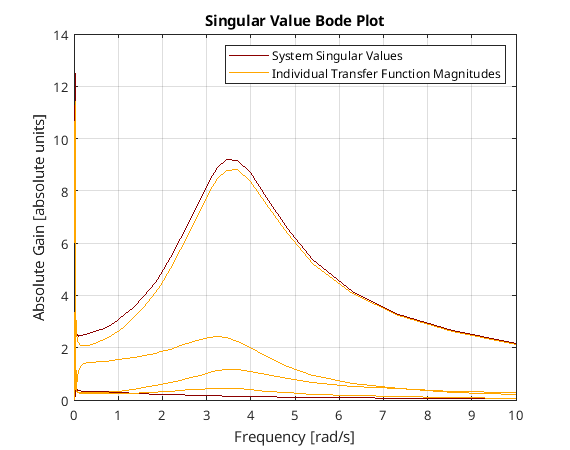
\includegraphics[width=\textwidth]{singularValuePlot.png}
\end{figure}

\subsection{}

\textit{From the plot in (a), estimate the worst case output 2-norm (in absolute units, not dB) for any $L_2[0, \infty)$ input signal with 2-norm equal to 1.}

There's a peak near 0 rad/s at about 12.5 if we take this as the max singular value then that would indicate the highest possible amplification of the input so the worst case for the output 2-norm for an input with 2-norm of 1 would be 12.5.

\subsection{}

\textit{For the frequency $\omega=10$ rad/s, what input direction is amplified most? (the MATLAB command evalfr is useful here)}

\begin{lstlisting}[style=matlabstyle]
phantomFreq = evalfr(phantomSS, 1i*10);
[U,S,V] = svd(phantomFreq);

disp('Most Amplified Input Direction: ');
disp(V(1,:));
\end{lstlisting}

I used the 'evalfr' function with 10 rad/s as shown above and then put that resulting frequency matrix through the 'svd' function and got $\begin{bmatrix}0.9913 \\ 0.1317\end{bmatrix}$ for the vector corresponding to the greatest singular value.
    
\section{}

\textit{In this problem you will design a feedback control for the thrust vector actuator for the RL10-B2 liquid rocket engine which is on the second stage of the Delta IV launch vehicle. The gimbal actuator takes an input voltage \(v(t)\) and rotates the nozzle an angle \(\phi(t)\), whose dynamics are described by}

\[
P(s) = \frac{\phi(s)}{v(s)} = \frac{40(s + 1)}{(s^2 + s + 4)(s + 6)}
\]

\textit{The desired closed loop system should have decent tracking behavior so that it can follow the reference command from the rocket’s guidance system. The system has a closed loop bandwidth constraint due to the large inertia of the nozzle and the limits of the gimbal actuator to rotate it. Assume the following specifications for your initial controller design:
\begin{itemize}
    \item Maximum closed loop bandwidth of 2 Hz (12.56 rad/s)
    \item Tracking error of less than 10\% from 0 to 0.5 Hz (3.14 rad/s)
    \item Closed loop step response with a maximum overshoot of 20\%
\end{itemize}
}

\subsection{}

\textit{Convert the closed loop performance requirements above into open loop constraints. Design a dynamic compensator \(C(s)\) and generate a bode plot of \(L(s) = P(s)C(s)\) that includes all the constraints so that you can visually verify that your design meets all performance requirements.}

For the maximum closed loop bandwidth of 12.56 rad/s we want the crossover point (the frequency where the open loop gain drops below 0dB) to be equal to the bandwidth frequency.
For the tracking error we want the open loop gain to be greater than 2 or 6dB, this is derived from the tracking error being equal to the magnitude of the sensitivity function which is the reciprocol of the open loop function.
For the overshoot we would like the phase margin to be 45.59 at the crossover point defined above, this is derived from the damping ratio formula $\zeta=(\frac{[ln(M_p)]^2}{\pi^2 + [ln(M_p)]^2})^{\frac{1}{2}}$ where $M_p$ is the max overshoot and the approximation that the phase margin is $100\cdot\zeta$ in degrees.

The plan is to begin by plotting the plant bode plot and then using my knowledge of the effects of compensators to adjust the system to our needs.
So I plotted the bode plot for the open loop transfer function and then looked at what and where needed to be modified.

\begin{figure}[H]
    \centering
    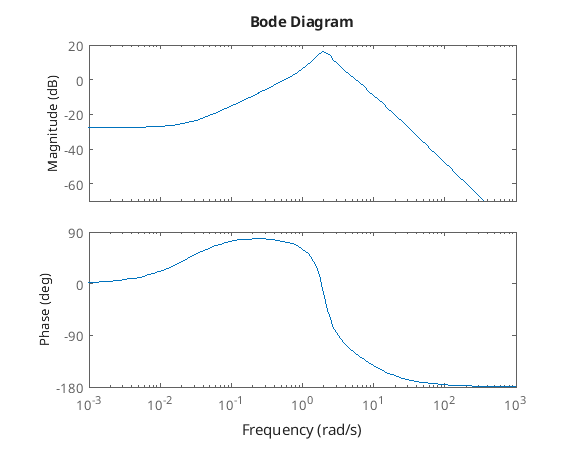
\includegraphics[width=0.75\textwidth]{delta4openPlot.png}
\end{figure}

I immediately noticed that the low frequency gain is negative and thought of the lag compensator to add gain specifically in those low frequencies.
Below is how I implemented it in Matlab, my thought was to keep alpha high to to start near/at zero and then at about the peak of the open loop to even it off again since I do want it to decline at some point and then I raised the whole curve by increasing k.

\begin{lstlisting}[style=matlabstyle]
k = 100;
alpha = 10000;
tau = 0.25;
numC1 = [k*tau k*1];
denC1 = [alpha*tau 1];
C1 = tf(numC1, denC1);    
\end{lstlisting}

Then I had to deal with the phase margin and so I introduced a lead compensator using a similar strategy except adjust alpha and tau to increase the phase around the area of the gain crossover.
The resulting lead/lag controller open loop bode plot is below:

\begin{figure}[H]
    \centering
    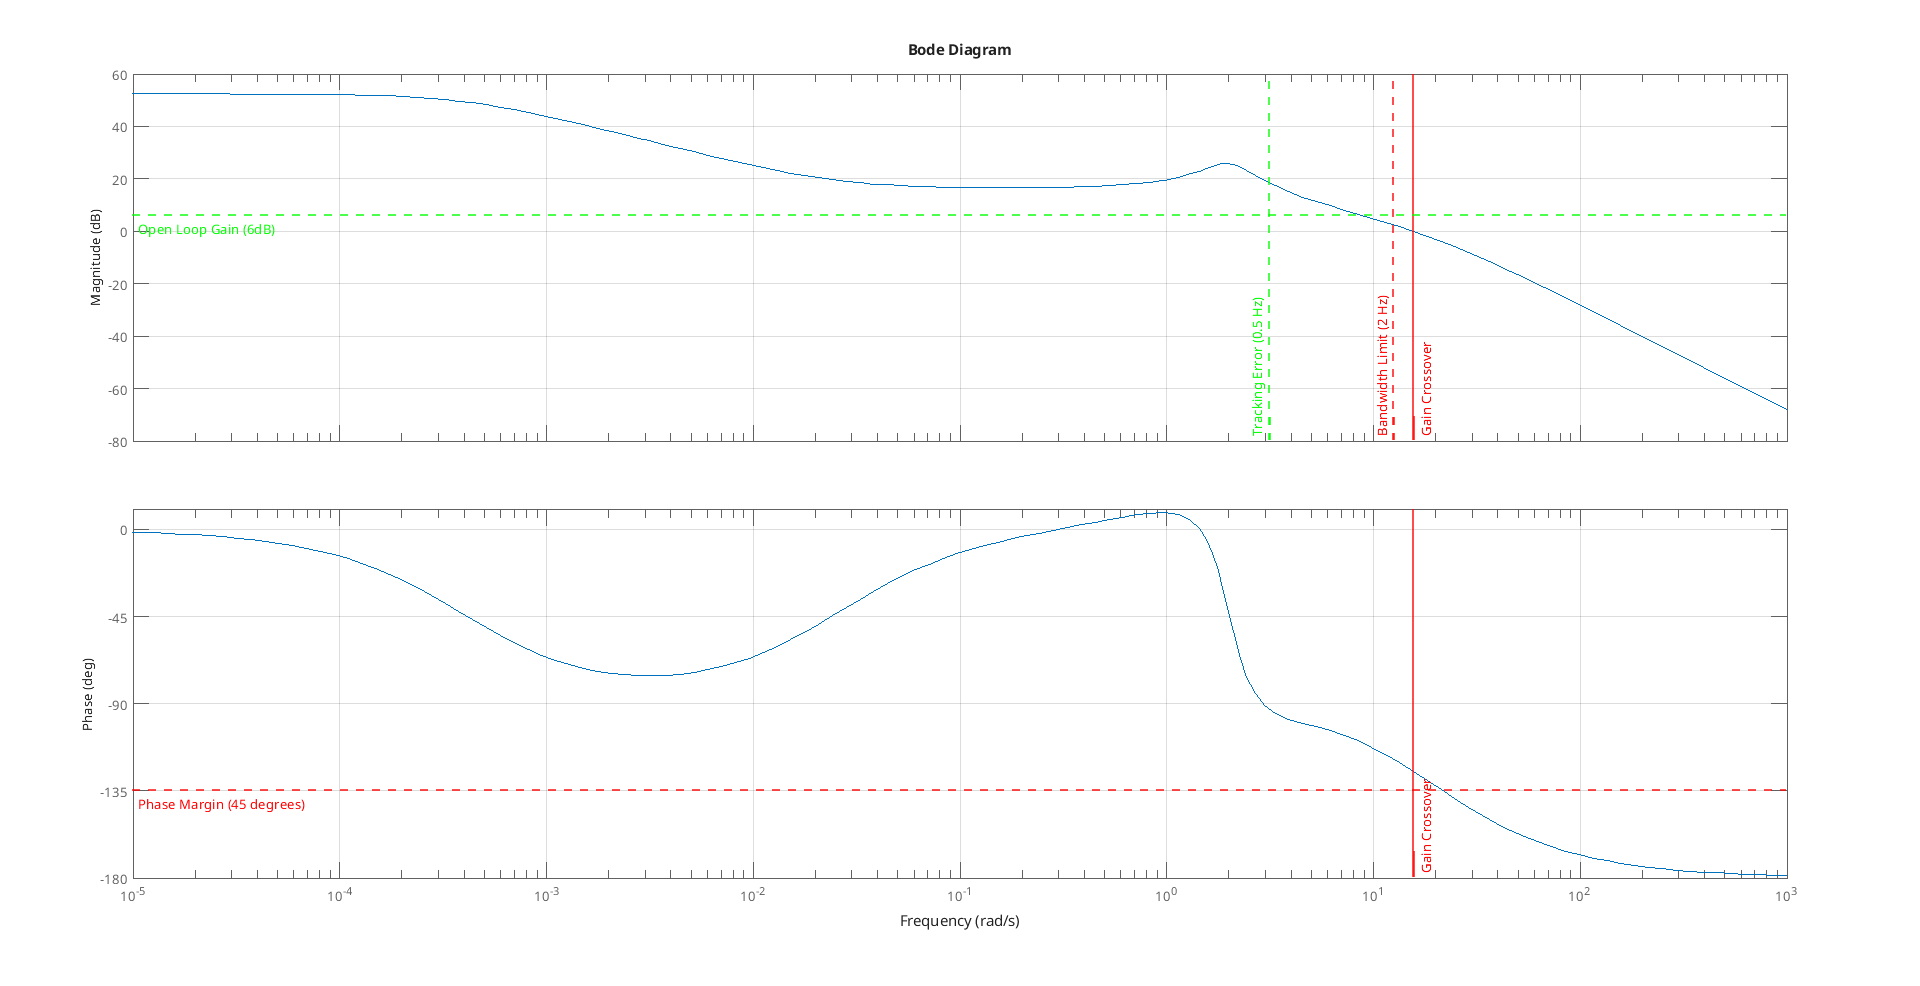
\includegraphics[width=\textwidth]{delta4leadLagPlot.png}
\end{figure}

I marked the tracking error specification in green and the other two in red so you can see how I met the specs.

\subsection{}

\textit{Generate a closed loop step response and error signal $e(t)$ for a reference input of $r = \sin(2\pi\omega t)$ for $\omega = 0.5$ Hz to show that the specs have been met.}

I generated the responses using 'step' and 'lsim' as well as generating the closed loop system using 'feedback'.
The results are below:

\begin{figure}[H]
    \centering
    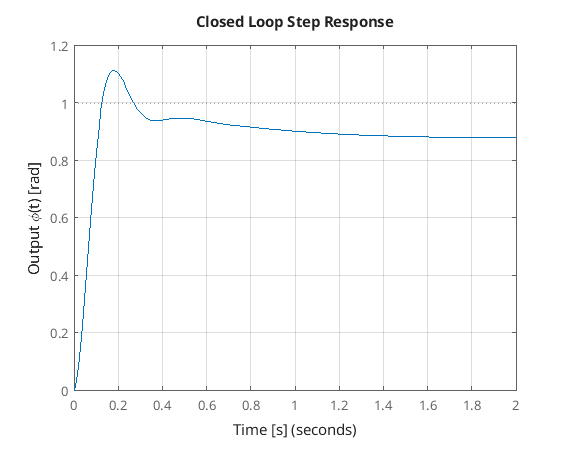
\includegraphics[width=\textwidth]{d4clStep.png}
\end{figure}

\begin{figure}[H]
    \centering
    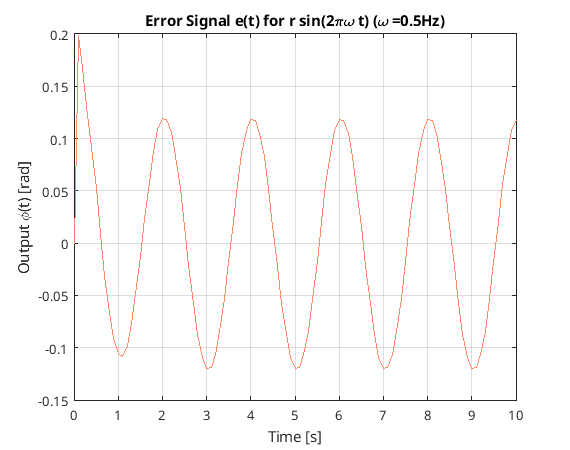
\includegraphics[width=\textwidth]{d4clSinError.png}
\end{figure}

And I plotted the sine input and response to show some extra perspective:

\begin{figure}[H]
    \centering
    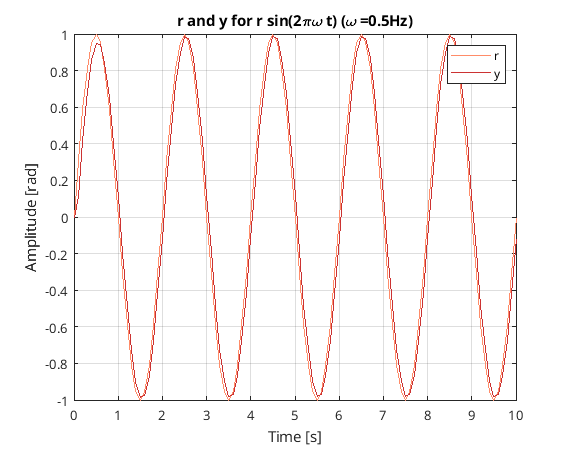
\includegraphics[width=\textwidth]{d4clRY.png}
\end{figure}

I think these pretty adequately show the max overshoot as you can see in the first plot that the response doesn't jump over 1.2 and in the second plot the error largely stays under 0.1. \\

\textit{After initial flight testing, it is determined that there are disturbances that effect the behavior of the system. Specifically, vibrations from the engine (high frequency) and fuel slosh (low frequency) were shown to have a significant impact. You are now to redesign your controller assuming that disturbances can arise from a large frequency range. Assume disturbances $d(t)$ that enter the loop at the plant input can be any signal with finite energy $d(t) \in L_2[0, \infty)$, and redesign your controller to minimize the effect on the output $\phi(t)$, which is also assumed to be a finite energy signal:}
    
\textit{- Maximum $||\phi||_2/||d||_2$ gain should be less than 1/3 (3X reduction)}

\subsection{}
\textit{Re-generate the open loop bode plot of $L(s) = P(s)C(s)$ with your new compensator that includes all the constraints so that you can visually verify that your design meets all the original performance requirements listed in the first part of the question.}

I started by generating the PS transfer function and plotting it and getting the $H_{\infty}$ norm and then adjusting the gain as needed.
I used 'feedback' and 'norm' to get the transfer function and $H_{\infty}$ norm.

\begin{lstlisting}[style=matlabstyle]
S = feedback(1,openLoop);
PS = plant*S;
disp(norm(PS, inf));
w = logspace(-1,3,1000);
[mag, ~] = bode(PS,w);
mag =squeeze(mag);
figure;
semilogx(w,mag,'Color', [255/255 140/255 105/255]);
hold on;
plot(w, 1/3*ones(size(w)), 'Color', [204/255 51/255 51/255]);
grid on;
title('Magnitude of PS at K = 100 [Absolute Units]');
xlabel('Frequency [rad/s]');
ylabel('Magnitude [abs]');
legend('PS', 'Max Gain 1/3');
hold off;    
\end{lstlisting}

The resulting $H_{\infty}$ norm was 0.3356 and the gain plot is below:

\begin{figure}[H]
    \centering
    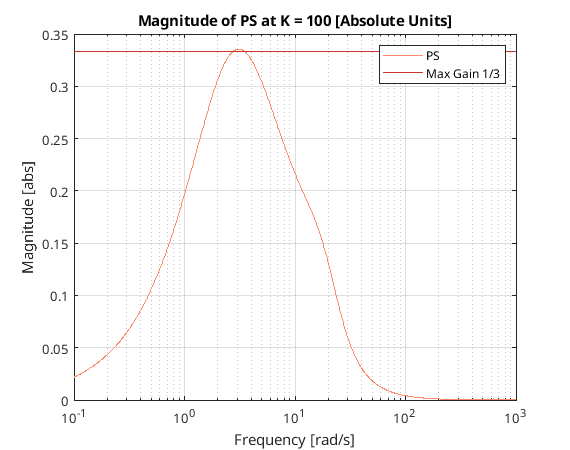
\includegraphics[width=\textwidth]{psk100.png}
\end{figure}

So you can see it already just dips above.
So I played with some gain values and landed on $K = 125$ that achieved the disturbance rejection I want while not changing the system enough that I had to adjust the compensators:

\begin{figure}[H]
    \centering
    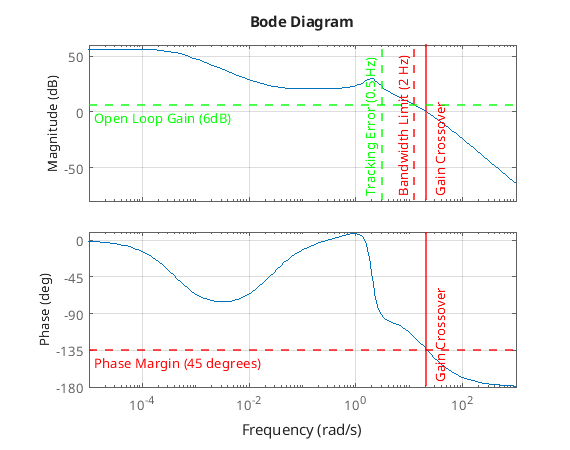
\includegraphics[width=\textwidth]{k125bode.png}
\end{figure}

\subsection{}
\textit{Generate a plot of the magnitude of the transfer function $PS(s)$ in absolute units to estimate the maximum $||\phi||_2/||d||_2$ gain and verify that you also satisfy this requirement (you can check this with the norm($PS$, inf)). along with a step and impulse response of $PS(s)$ to visualize the effect of the disturbance on your system.}

The $H_{\infty}$ norm became 0.2153 ('norm' function).
Here is the magnitude plot:

\begin{figure}[H]
    \centering
    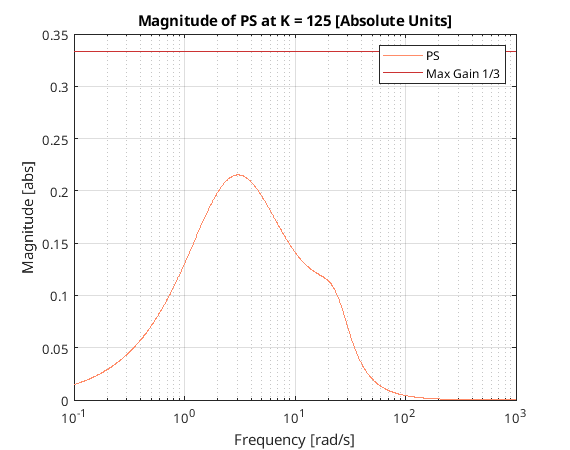
\includegraphics[width=\textwidth]{psk125.png}
\end{figure}

And below are the step and impulse response from disturbance to output:

\begin{figure}[H]
    \centering
    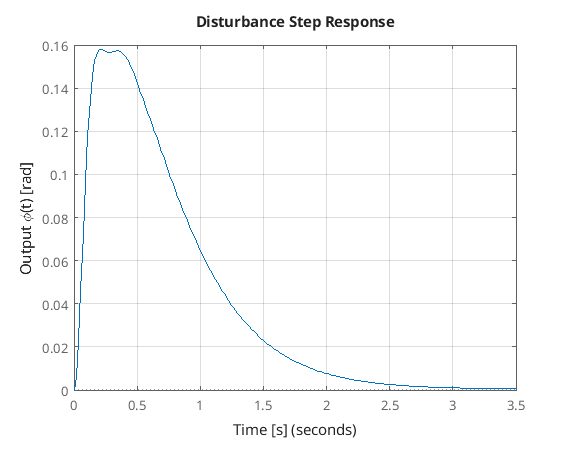
\includegraphics[width=\textwidth]{step125.png}
\end{figure}

\begin{figure}[H]
    \centering
    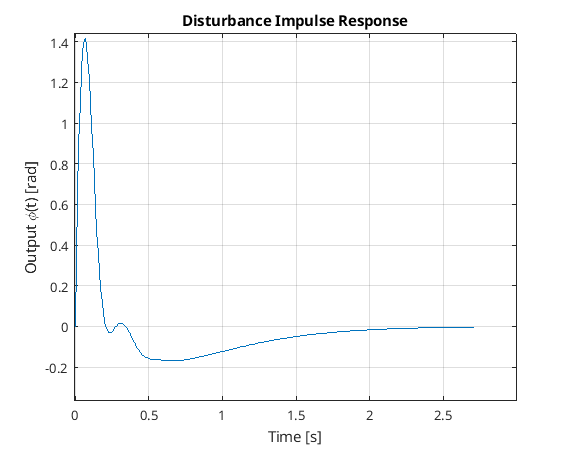
\includegraphics[width=\textwidth]{impulse125.png}
\end{figure}

\end{document}